%
% loesung.tex -- Loesung Kalman-Filter
%
% (c) 2006-2015 Prof. Dr. Andreas Mueller, Hochschule Rapperswil
%

\section{Lösung für das Filterproblem}
\kopfrechts{Lösung für das Filterproblem}
Zur Zeit $k$ ist das System im Zustand $x_k$, von dem uns aber nur die
Schätzung $\hat x_k$ bekannt ist.
Anschliessend wird sich
das System entsprechend der Zeitentwicklungsgleichung entwickeln und
so den Zustand $x_{k+1}$ erreichen.
Auch diesen Zustand können wir nicht
kennen, es genügt, eine Schätzung davon zu bestimmen.
Dies kann in zwei
Schritten geschehen:
\begin{enumerate}
\item Man überlässt das System sich selbst, und versucht eine möglichst
gute Schätzung für den Zustand $x_{k+1}$ zu finden, die nur auf dem
Wissen zur Zeit $k$ basiert.
Wir schreiben dafür $\hat x_{k+1|k}$.
\item Mit Hilfe der Messung $z_{k+1}$, die zur Zeit $k+1$ stattfindet, wird
$\hat x_{k+1|k}$ zu einer optimalen Schätzung zur Zeit $k+1$ verfeinert.
\end{enumerate}
Tabellarisch können wir die Schritte wie folgt darstellen:
\[
\xymatrix @-1mm {
k\ar[dd]&x_k\ar[dd]\ar[dd]^{\varphi_k, u_k} &\hat x_k\ar[d]^{\varphi_k}      &P_{k} \ar[d]^{\varphi_k,Q_k}    \\
        &           &\hat x_{k+1|k}\ar[d]^{H_k,K_k}&P_{k+1|k}\ar[d]^{R_k,H_k\Rightarrow K_k} \\
k+1     &x_{k+1}    &\hat x_{k+1}  &P_{k+1}
} \]
Die Pfeile sind mit den Matrizen angeschrieben, die bei den einzelnen Schritten zum
Einsatz kommen werden.

\subsection{Voraussage}
\index{Kalman-Filter!Vorhersage-Schritt}
\begin{figure}
\centering
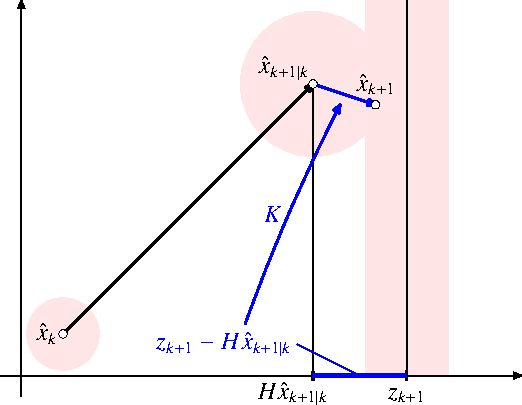
\includegraphics{images/filter-2.pdf}
\caption{Vorhersage und Messung mit ihren jeweiligen Fehlern geben eine
korrigierte Vorhersage höherer Genauigkeit
\label{bild-vorhersage-korrektur}}
\end{figure}
Überlässt man das System sich selbst, wird es sich gemäss der
Entwicklungsgleichung entwickeln.
Allerdings ist uns der Systemfehler
$u_k$ nicht bekannt, die einzige Schätzung, die uns auf der Basis dieser
Informationen möglich ist, ist also
\[
\hat x_{k+1|k}=\varphi_k\hat x_k
\]
In Abbildung~\ref{bild-vorhersage-korrektur} ist die Vorhersage schematisch
dargestellt, zusammen mit ihren Fehlern.

Wir wollen nicht nur $\hat x_k$ zu jeder Zeit bestimmen können, sondern
auch eine Information über die Fehler mitberechnen, also die Fehlerkovarianzmatrix
nachführen.
Wir berechnen daher auch $P_{k+1|k}$
\begin{align*}
P_{k+1|k}&=E(\tilde x_{k+1|k}\tilde x_{k+1|k}^t)\\
&=E( (\hat x_{k+1|k}-x_{k+1} ) (\hat x_{k+1|k}-x_{k+1} )^t)\\
&=E(
(\varphi_k\hat x_k-\varphi_kx_k-u_k)
(\dots)^t
)\\
&=E(
(\varphi_k(\hat x_k-x_k)-u_k)
(\dots)^t
)\\
&=E(
(\varphi_k(\tilde x_k)-u_k)
(\dots)^t
)\\
&=E(
(\varphi_k(\tilde x_k)-u_k)
(\tilde x_k^t\varphi_k^t-u_k^t)
)\\
&=E(\varphi_k\tilde x_k \tilde x_k^t\varphi_k^t)-E(u_k\tilde x_k\varphi_k^t)-E(\varphi_k\tilde x_ku_k)+E(u_ku_k^t)\\
&=\varphi_k E(\tilde x_k \tilde x_k^t)\varphi_k^t-E(u_k\tilde x_k)\varphi_k^t-\varphi_k E(\tilde x_ku_k)+E(u_ku_k^t)\\
&=\varphi_kP_k\varphi_k^t+Q_k
\end{align*}
Damit haben wir einen Formelsatz, mit dem der erste Teilschritt zur Berechnung
der Schätzung zur Zeit $k+1$ möglich ist:
\begin{definition}Der Voraussageschritt für das Filterproblem wird durch
\begin{align}
\hat x_{k+1|k}&=\varphi_k\hat x_k \label{estimate-prediction}\\
P_{k+1|k}&=\varphi_kP_k\varphi_k^t + Q_k \label{covariance-prediction}
\end{align}
berechnet.
\end{definition}

\subsection{Korrektur}
\index{Kalman-Filter!Korrekturschritt}
Im zweiten Schritt wird jetzt aus der provisorischen Schätzung $\hat x_{k+1|k}$
und der Messung $z_{k+1}$ die definitive Schätzung zur Zeit $k+1$ berechnet.
Ebenfalls nachgeführt werden muss die Fehlerkovarianzmatrix $P_{k+1}$.
In Abbildung~\ref{bild-vorhersage-korrektur} ist auch die Korrektur auf der Basis
der Messung $z_{k+1}$ dargestellt, so entsteht eine neue Schätzung
$\hat x_{k+1}$ höherer Präzision.

In den folgenden Herleitungen kommt vor allem der Index $k+1$ vor.
Um die Formeln
etwas zu vereinfachen, erhöhen wir jetzt $k$ um eins, d.~h.~wir können
überall $k+1$ durch $k$ und $k$ durch $k-1$ ersetzen.

Da der Schätzer linear sein soll, und nur von $\hat x_{k|k-1}$ und $z_{k}$
abhängen soll, setzen wir ihn mit Hilfe der zwei Matrizen $K_k'$ und $K_k$
wie folgt an:
\[
\hat x_{k}=K_{k}' \hat x_{k|k-1}+K_{k} z_{k}.
\]
Die Matrizen $K_{k}'$ und $K_{k}$ sollen jetzt so bestimmt werden, dass der Schätzer
$\hat x_{k}$ gute Eigenschaften hat.

Zunächst möchten wir sicherstellen, dass der Schätzer erwartungstreu ist,
oder, was auf das gleiche hinausläuft, dass der Erwartungswert des Fehlers
$\tilde x_{k}=\hat x_{k}-x_{k}$ verschwindet.
Wir berechnen den Fehler
mit Hilfe der Formel für $\hat x_{k}$
\begin{align*}
\tilde x_{k}&=\hat x_{k}-x_{k}\\
&=K_{k}'\hat x_{k|k-1}+K_{k}z_{k}-x_{k}\\
&=K_{k}'\hat x_{k|k-1}+K_{k}H_{k}x_{k} + K_{k}w_{k}-x_{k}\\
&=K_{k}'\hat x_{k|k-1}+K_{k}H_{k}x_{k} -x_{k} + K_{k}w_{k}\\
&=K_{k}'(\tilde x_{k|k-1}+x_{k})+K_{k}H_{k}x_{k}-x_{k}+K_{k}w_{k}\\
&=(K_{k}'+K_{k}H_{k}-I)x_{k}+K_{k}'\tilde x_{k|k-1}+K_kw_k
\end{align*}
Daraus berechnet man den Erwartungswert des Fehlers
\begin{align*}
E(\tilde x_{k})&=(K_{k}'+K_{k}H_{k}-I)E(x_{k})+K_{k}'E(\tilde x_{k|k-1})+K_{k}E(w_{k})\\
&=(K_{k}'+K_{k}H_{k}-I)E(x_{k})
\end{align*}
weil $\tilde x_{k|k-1}$ bereits erwartungstreu ist und $E(w_{k})=0$ nach Voraussetzung.
Dies verschwindet nur dann immer, wenn die Matrix in Klammern $0$ ist,
also
\[
K_{k}'+K_{k}H_{k}-I=0\qquad\Rightarrow\qquad K_{k}'=I-K_{k}H_{k}.
\]
Somit ist $K_{k}'$ durch die Bedingung der Erwartungstreue eindeutig bestimmt.
Mit dieser Wahl von $K_{k}'$ wird der Schätzer jetzt
\[
\hat x_{k}=(I-K_{k}H_{k})x_{k|k-1}+K_{k}z_{k}.
\]

Die zweite Bedingung ist, dass die Fehlerkovarianzmatrix möglichst klein wird,
daher berechnen wir zunächst $\tilde x_{k}$:
\begin{align*}
\tilde x_{k}&=\hat x_{k}-x_{k}\\
&=(I-K_{k}H_{k})\hat x_{k|k-1}+K_{k}z_{k}-x_{k}\\
&=(I-K_{k}H_{k})\hat x_{k|k-1}+K_{k}H_{k}x_{k}+K_{k}w_k-x_{k}\\
&=(I-K_{k}H_{k})\tilde x_{k|k-1}+K_{k}w_k
\end{align*}
Somit ist $\tilde x_{k}$ durch $\tilde x_{k|k-1}$ ausgedrückt, damit sollten
wir $P_{k}$ aus $P_{k|k-1}$ berechnen können:
\begin{align*}
P_{k}&=E(\tilde x_{k}\tilde x_{k}^t)\\
&=E(
((I-K_{k}H_{k})\tilde x_{k|k-1}+K_{k}w_k)
(\dots)^t
)\\
&=(I-K_{k}H_{k})P_{k|k-1}(I-K_{k}H_{k})^t\\
&\quad +(I-K_{k}H_{k})E(\tilde x_{k|k-1}w_k^t)K_{k}^t\\
&\quad+K_{k}E(w_k\tilde x_{k|k-1}^t)(I-K_{k}H_{k})\\
&\quad+K_{k}E(w_kw_k^t)K_{k}^t\\
&=(I-K_{k}H_{k})P_{k|k-1}(I-K_{k}H_{k})^t +K_{k}R_kK_{k}^t
\end{align*}
Diese Formeln bilden nun auch den zweiten Schritt, offen ist nur noch die
geeignete Wahl der Matrix $K_{k}$.
\begin{definition}
Der Korrekturschritt im Filterproblem ist gegeben durch
\begin{align}
\hat x_{k}&=(I-K_{k}H_{k})x_{k|k-1}+K_{k}z_{k} \label{estimate-correction}\\
P_{k} &=(I-K_{k}H_{k})P_{k|k-1}(I-K_{k}H_{k})^t +K_{k}R_kK_{k}^t \label{covariance-correction}
\end{align}
\end{definition}

\subsection{Der optimale Filter}
\index{Kalman-Filter!optimaler Filter}
Die Zeitentwicklung des Schätzers kann nun bis auf die unbekannte Matrix $K_k$
berechnet werden.
Es bleibt, $K_k$ zu bestimmen.
$K_k$ soll so gewählt werden,
dass die Spur von $P_{k}$ minimal wird.
Dabei können wir verwenden,
dass $P_{k}$ von der Form $ABA^t$ ist, wobei $B$ eine symmetrische
Matrix ist.
Für solche Matrizen ist die Ableitung nach den Komponenten
$A$ leicht zu berechnen, das Minimum von $\operatorname{tr}(ABA^t)$
kann daher durch Nullsetzen der Ableitung gefunden werden.

\begin{hilfssatz}Ist $B$ eine symmetrische Matrix und $A$ eine beliebige
Matrix, dann ist die Matrix der Ableitungen von $\operatorname{tr}(ABA^t)$
nach den Komponenten von $A$  ist $2AB$.
\end{hilfssatz}

\begin{proof}[Beweis]
Es ist
\[
\operatorname{tr}(ABA^t)=\sum_{i,j,k}a_{ij}b_{jk}a_{lk}.
\]
Ableiten nach $a_{uv}$ ergibt:
\[
\frac{\partial}{\partial a_{uv}}\operatorname{tr}(ABA^t)
=\sum_{k}b_{vk}a_{uk}+\sum_{j}a_{uj}b_{jv}
\]
Die zwei Terme auf der rechten Seite unterscheiden sich nur durch
die Bezeichnung für die Laufvariable, also
\[
\frac{\partial}{\partial a_{uv}}\operatorname{tr}(ABA^t)
=(2AB)_{uv}.
\]
\end{proof}

Angewendet auf $P_{k}$ bedeutet dies, dass für das optimale $K_k$
\[
-(I-K_kH_{k})P_{k|k-1}H_{k}^t +K_kR_k=0
\]
verlangt werden muss.
Dies kann man nach $K_k$ auflösen und findet
\begin{align*}
0&=-P_{k|k-1}H_{k}^t +K_k[H_{k}P_{k|k-1}H_{k}^t +R_{k}]\\
P_{k|k-1}H_{k}^t&=K_k[H_{k}P_{k|k-1}H_{k}^t +R_{k}]\\
K_k&= P_{k|k-1}H_{k}^t [H_{k}P_{k|k-1}H_{k}^t +R_{k}]^{-1}
\end{align*}
Damit ist das Filterproblem eigentlich vollständig gelöst.
Wir bemühen uns
aber noch, mit der Lösung für $K_k$ die Berechnung der Fehlerkovarianz etwas zu
vereinfachen.
Es gilt
\begin{align*}
P_{k}&=(I-K_{k}H_{k})P_{k|k-1}(I-K_{k}H_{k})^t+K_{k}R_kK_{k}^t\\
&=P_{k|k-1} + K_{k}(H_{k}P(-)H_{k}^t+R_k)K_{k}^t -K_{k}H_{k}P_{k|k-1}-P_{k|k-1}H_{k}^tK_{k}^t\\
&=P_{k|k-1} - P_{k|k-1}H_{k}^t(H_{k}P_{k|k-1}H_{k}^t+R_k)^{-1}H_{k}P_{k|k-1}\\
&=(I-P_{k|k-1}H_{k}^t(H_{k}P_{k|k-1}H_{k}^t + R)^{-1}H_{k})P_{k|k-1}\\
&=(I-K_{k}H_{k})P_{k|k-1}\\
\end{align*}
Damit können wir das Resultat zusammenstellen:
\begin{satz}
Der beste lineare Schätzer für das Filterproblem wird durch die Kalman-Matrix
$K_k$ gegeben, welche mittels
\begin{equation}
K_k=P_{k|k-1}H_k^t(H_kP_{k|k-1}H_k^t+R_k)^{-1}
\label{kalman-gains}
\end{equation}
berechnet wird.
Das Fehlerkovarianz-Update wird mit der Kalman-Matrix
vereinfacht zu
\[
P_k=(I-K_kH_k)P_{k|k-1}.
\]
\end{satz}

\subsection{Datenfluss}
\begin{figure}
\[
\xymatrix @-1mm {
&u_k\ar[r]& *+[o][F]{+}\ar[ddd]_{x_k}&                               \\
&&                   & *+[F]{\varphi_{k-1}}\ar `u^l[ul] [ul]          \\
*\txt{unbeobachtetes System}&&                   & *+[F]\txt{DELAY} \ar[u]       \\
&& *{\bullet}\ar[dd]\ar `r^u[ru] [ru]         &                        \\
\ar@{.}[rrr]&&&\\
*\txt{Messung}&& *+[F]{H_k}\ar[d] & \\
&w_k\ar[r]& *+[o][F]{+}\ar[dd]_<<<<{z_k} &                      \\
\ar@{.}[rrr]&&&\\
&& *+[o][F]{-}\ar[d]_{z_k-H_k \hat x_{k|k-1}} &                               \\
&& *+[F]{K_k}\ar[d]  & *+[F]{H_k}\ar `u^l[ul] [ul]   \\
*\txt{Kalman-Filter}&& *+[o][F]{+}\ar[ddd]_{\hat x_k}  & *{\bullet}\ar[u]\ar[l]\\
&&                   & *+[F]{\varphi_{k-1}}\ar[u]^{\hat x_{k|k-1}}            \\
&&                   & *+[F]\txt{DELAY} \ar[u]       \\
&& *{\bullet}\ar `r^u[ru] [ru] \ar[d]&                     \\
&& \hat x_k          &                               \\
}\]
\caption{Datenfluss im Kalman-Filter\label{datenfluss}}
\end{figure}
\begin{figure}
\[
\xymatrix @-1mm {
*+[F]{H_{k-1}}\ar [rd] & & \\
&*+[F]\txt{Berechne $P_{k-1}$ nach (\ref{covariance-correction})}\ar[ddd]&\\
*+[F]{R_{k-1}}\ar[ur] & & \\
*+[F]{\varphi_{k-1}}\ar[dr] & & \\
&*+[F]\txt{Berechne $P_{k|k-1}$ nach (\ref{covariance-prediction})} \ar[dd] & &\\
*+[F]{Q_{k-1}} \ar[ur] & & \\
&*[F]\txt{\strut Berechne $K_k$ nach (\ref{kalman-gains})} \ar[d] && \\
&*{\bullet} \ar `r^u[r] `u^l[ruuuuuuu]_{\text{erhöhe }k} `l^d[uuuuuuu] [uuuuuu] \ar[d]&&\\
&&&\\
}\]
\caption{Berechnung der Kalman-Matrix\label{k-berechnung}}
\end{figure}
Abbildung \ref{datenfluss} zeigt den Datenfluss für den Kalman Filter.
Im oberen Teil des Diagramms ist das `unbeobachtete' System mit seiner
Zeitentwicklung und den Systemfehlern $u_k$ dargestellt.
Unterhalb der
punktierten Linie folgt die Messung, die Matrix $H_k$ reduziert den Zustand
auf diejenigen Grössen, die durch die Messung zugänglich werden, und es
werden die Messfehler $w_k$ hinzugefügt.
Beide Teile sind nur für die
mathematische Beschreibung des Kalman-Filters notwendig, sie werden
sozusagen von der Natur und den Sensoren realisiert.

Die untere Hälfte zeigt den eigentlichen Kalman-Filter.
Aus einem frühren Zustand $\hat x_{k-1}$ wird mit Hilfe der Matrix
$\varphi_k$ eine provisorische Schätzung $\hat x_{k|k-1}$ erstellt.
Mit der Matrix $H_k$ wird darauf eine Messung simuliert.
Diese wird
mit der tatsächlichen Messung verglichen und die Differenz, verstärkt durch
die Kalman-Matrix $K_k$ zur provisorischen Schätzung hinzugefügt, was
die definitive neue Schätzung $\hat x_k$ für $x_k$ ergibt.

In Abbildung \ref{k-berechnung} ist der Datenfluss für die Berechnung
der Fehlerkovarianzmatrix und der Kalman-Matrix dargestellt.

\subsection{Spezialfälle}
Sind die Matrizen konstant, die das System und den Messprozess beschreiben, 
dann werden im Prozess nach Abbildung \ref{k-berechnung} sowohl $P_k$ also auch
$K_k$ oft gegen konstante Matrizen konvergieren.
In diesem Fall kann man
die Matrix $K=\lim_{n\to\infty}K_n$ vorgängig berechnen, und braucht
in der Implementation des Filters die Berechnung der Fehlerkovarianzmatrix
gar nicht mehr mitzuberechnen. 

Wir betrachten den Spezialfall eines konstanten System mit genau einer
Zustandsvariable,
die auch gemessen wird.
Man erwartet keine Änderung der Zustandsvariable,
die Matrix $\varphi$ ist also die Einheitsmatrix.
Der Voraussageschritt wird
dann zu 
\begin{align*}
\hat x_{k|k-1}&=\hat x_{k-1}\\
P_{k|k-1}&=P_{k-1}+Q,
\end{align*}
die Kalman-Matrix 
\[
K_{k}=\frac{P_{k|k-1}}{P_{k|k-1}+R}=\frac{P_{k-1}+Q}{P_{k-1}+Q+R},
\]
und das Update der Fehlerkovarianz damit zu
\begin{align*}
P_k&=(1-K_k)P_{k|k-1}\\
&=\frac{R(P_{k-1}+Q)}{P_{k-1}+Q+R}
\end{align*}
Diese Gleichung hat tatsächlich einen Fixpunkt, den man durch
Einsetzen von $P=P_k=P_{k-1}$ findet:
\[
P=\frac{R(P+Q)}{P+Q+R}
\quad\Rightarrow\quad
P^2+QP-QR=0
\quad\Rightarrow\quad
P=\frac{Q}2+\sqrt{\frac{Q^2}4+RQ}
\]
Damit kann man nun auch einen geschlossenen Ausdruck für $K$
finden:
\[
K=\frac{1}{1+R\biggl(\displaystyle\frac{Q}2+\sqrt{\frac{Q^2}4+RQ}\biggr)^{-1}}
=\frac1{1+R/P}
\]
Wir beobachten darin folgende Grenzfälle:
\begin{enumerate}
\item Ist $R=0$, also keine Messfehler, dann ist $K=1$.
Da die Vorhersage
$\hat x_{k|k-1}=\hat x_k$ ist, bedeutet dies, dass Abweichungen des Messwertes
von der Vorhersage vollständig in den neuen Messwert übernommen werden,
der Kalmanfilter reproduziert also die Messwerte exakt.
\item Im Grenzfall $Q=0$ erhalten wir $P=0$ und damit auch $K=0$.
Dies
bedeutet, dass der Filter überhaupt nicht mehr auf die Messungen reagiert,
der einmal ermittelte Schätzwert ist bereits die beste mögliche Schätzung.
\item Für einen Zwischenwert ergibt sich ein Wert von $K$ zwischen $0$ und $1$.
Nehmen wir als Beispiel an, dass die Messwerte bei $k_0$ einen Sprung machen,
danach aber konstant sind, dann wird der Schätzwert gegen den neuen Messwert
konvergieren.
Die Abweichung zwischen Messwert und vorhergesagtem Wert wird
in jeder Iteration mit $K$ multipliziert.
Bei einem kleinen Wert von $K$
kann der Filter einer Änderung rascher folgen, dafür wird auch $P$ entsprechend
gross, die Schätzung ist also nicht besonders zuverlässig.
Umgekehrt wird der Filter mit $K$ nahe bei $1$ träge, dafür kann dann auch
$P$ kleiner sein, die Schätzungen des Filters sind präziser.
\end{enumerate}
Auch im allgemeinen Fall eines konstanten Systems kann man erwarten,
dass bei einem Sprung der Inputdaten der Filter eine Abweichung vom
wahren Wert zeigt, welche exponentiell zerfällt.

